\documentclass[a4paper,12pt]{report}
\usepackage{geometry} % Для последующего задания полей
\geometry{a4paper,top=15mm,bottom=20mm,left=10mm,right=10mm}
\usepackage[T2A]{fontenc}	     % Поддержка русских букв
\usepackage[utf8]{inputenc}	     % Кодировка utf8
\usepackage[english, russian]{babel} % Языки: русский, английский
\usepackage{graphicx}                % Подключаем пакет работы с графикой

\renewcommand{\arraystretch}{1.3}

\begin{document}


\section*{Исходные данные}

\begin{table}[h!]
  \renewcommand{\tabcolsep}{0.9em}
  \centering
  \begin{tabular}{cccccccccc}
    (-0.68; -0.26)	& (-4.03; -2.32)	& (-0.72; 0.47)	& (1.25; 0.82)	& (1.27; -0.81)	\\ 
(-3.57; 0.46)	& (3.00; -2.85)	& (-2.19; 2.71)	& (-4.72; 0.48)	& (4.38; 2.77)	\\ 
(1.16; 2.37)	& (-1.04; 2.03)	& (-0.63; 1.74)	& (-0.07; -0.30)	& (-1.55; 1.85)	\\ 
(1.57; -0.10)	& (-0.27; -0.84)	& (-1.92; -0.17)	& (-0.80; -0.27)	& (-0.30; 3.87)	\\ 
(-2.51; -1.20)	& (0.21; 0.36)	& (2.99; 2.78)	& (2.26; 2.43)	& (1.95; 0.79)	\\ 
(3.27; 0.62)	& (-0.40; 2.71)	& (-0.53; 1.01)	& (0.16; 2.11)	& (3.07; 0.47)	\\ 
(-0.87; -2.17)	& (2.41; -0.85)	& (-0.52; -1.54)	& (0.99; -0.26)	& (0.57; 1.41)	\\ 
(1.47; -0.41)	& (5.76; -1.11)	& (-1.16; 0.95)	& (-1.22; -3.60)	& (3.13; 2.46)	\\ 
(0.90; 0.79)	& (0.77; -3.32)	& (-0.80; -1.46)	& (1.48; -0.69)	& (0.18; 0.25)	\\ 
(2.08; 2.50)	& (-0.99; -2.73)	& (-1.33; 1.70)	& (-2.36; -2.75)	& (-1.82; -2.29)	\\ 
	\\ 

  \end{tabular}
  \caption{Исходная выборка}
\end{table}

\section*{Линия регрессии}

\begin{figure}[h!] 
  \centering
  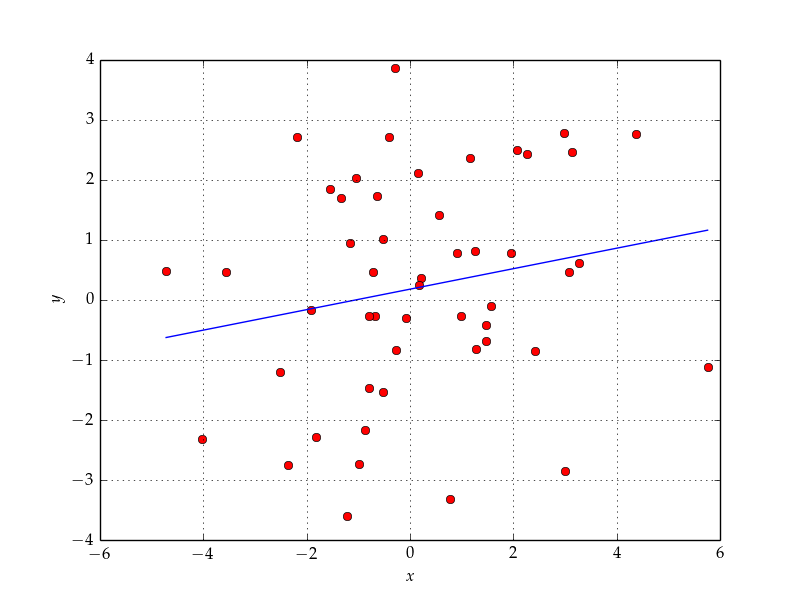
\includegraphics[width=0.8\linewidth]{../pic/sample_regression}
  \caption{График линии регрессии для заданной выборки}
\end{figure}


\end{document}